\documentclass{article}
\usepackage{graphicx} % Required for inserting images
\usepackage{booktabs}
\usepackage{float}
\usepackage{amsmath}
\title{Lesson 1 Homework - Calculus}
\author{William Wang}
\date{August 2026}

\begin{document}

\maketitle

\section{}
\subsection{}
We have 
\[s(t) = \sqrt{2t+1}\]
then
\[\text{avg velocity on interval } [3,5] = \frac{\Delta s}{\Delta t} = \frac{s(5)-s(3)}{2} = 
\frac{\sqrt{11}-\sqrt{7}}{2} \]
\subsection{}
\[v(h) = \frac{\Delta s}{\Delta t} = \frac{s(4+h) - s(4)}{h} = \frac{\sqrt{9+2h} - \sqrt{9}}{h}\]
\subsection{}
\begin{table}[h]
\centering
\begin{tabular}{cc}
\toprule
$h$ & $v(h)$ \\
\midrule
$-0.1$    & $0.335206$ \\
$-0.01$   & $0.333519$ \\
$-0.001$  & $0.333352$ \\
$-0.0001$ & $0.333335$ \\

$0.0001$& $0.333328$ \\
$0.001$   & $0.333315$ \\
$0.01$    & $0.333148$ \\
$0.1$     & $0.331502$ \\
\bottomrule
\end{tabular}
\end{table}
This shows that 
\[\lim_{h\to 0} v(h) = \frac{1}{3}\]
This limit represents the instantaneous velocity at \(t = 4\). 
\subsection{}
\begin{figure}[H]
    \centering
    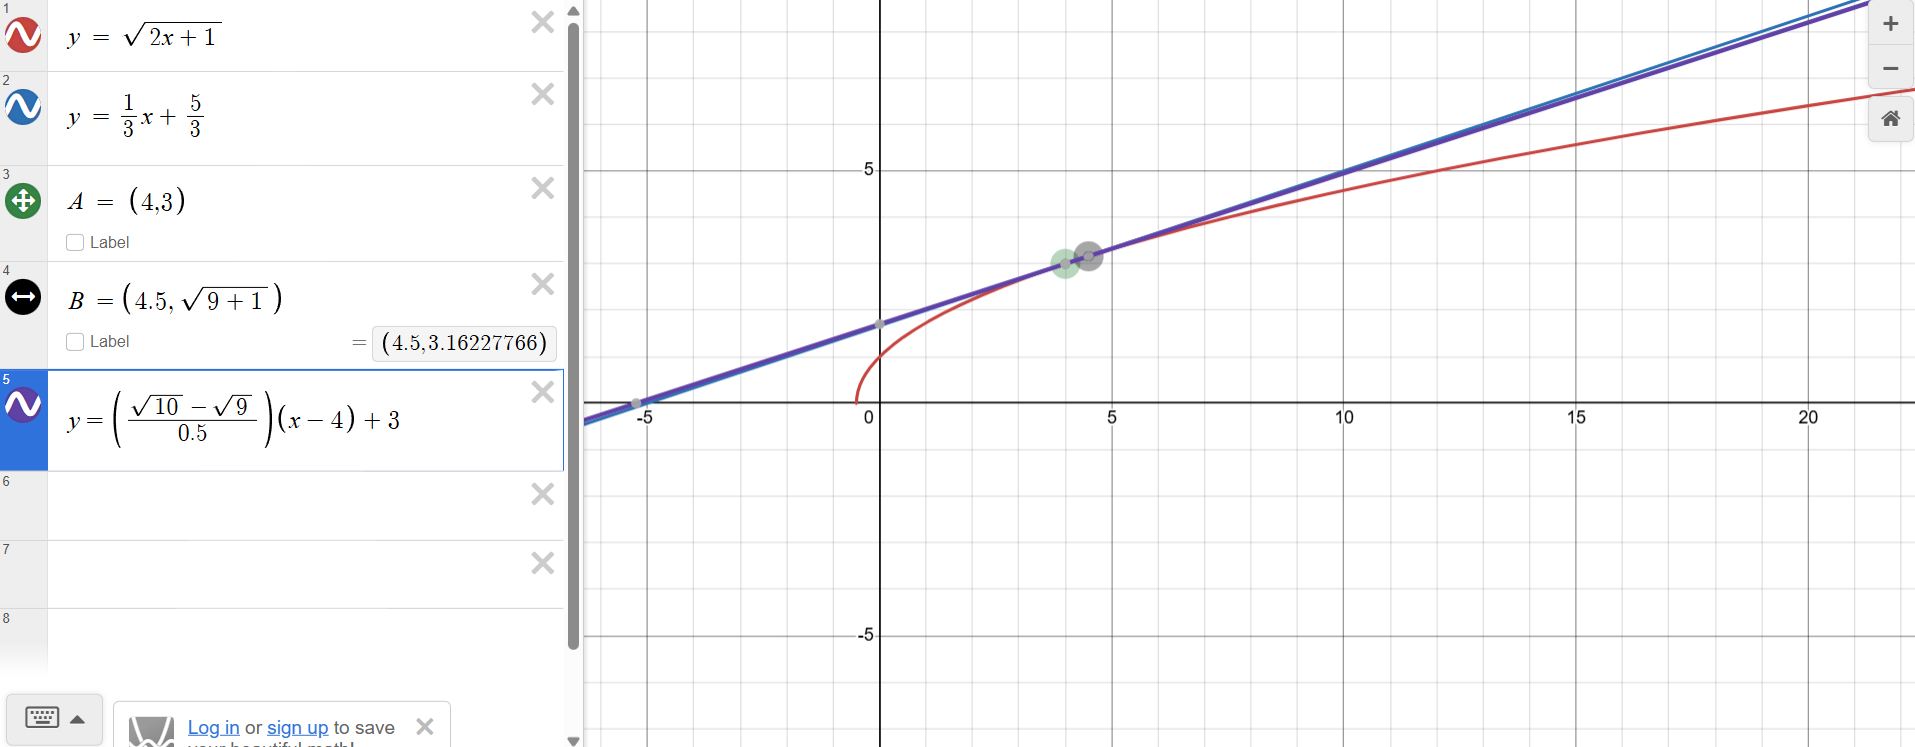
\includegraphics[width=1\linewidth]{6.png}

\end{figure}
The purple line is the secant line while the blue is the tangent line. The slope of the secant line should be the average velocity with \(h = 0.5\). Hence it should join \((4,s(4))\) and \((4.5, s(4.5))\). 
\subsection{}
Since we have the slope \(m = \frac{1}{3}\), therefore the equation of the tangent line is 
\[y - 3 = \frac{1}{3}(x-4)\]
\[y = \frac{1}{3}x+\frac{5}{3}\]
This tangent line has the same slope as the limit we found in part c.
\subsection{}
They look identical. The tangent line is the best approximation because if we zoom in enough, the curve and the tangent line become almost indistinguishable meaning we can use the tangent line's slope to find the curve's instantaneous rate of change at that point. 
\begin{figure}[H]
    \centering
    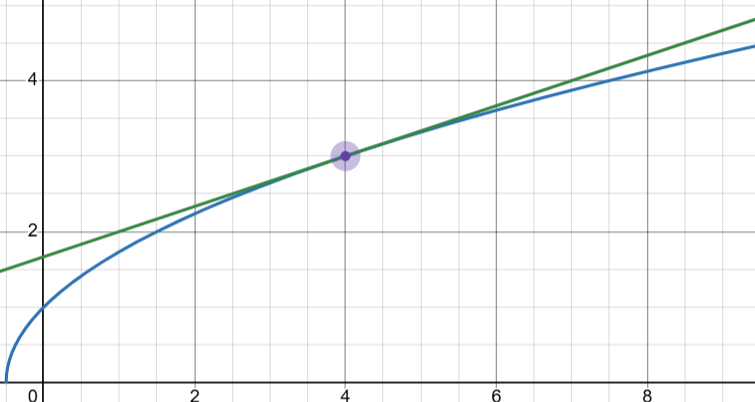
\includegraphics[width=0.5\linewidth]{image.png}
    
\end{figure}
\begin{figure}[H]
    \centering
    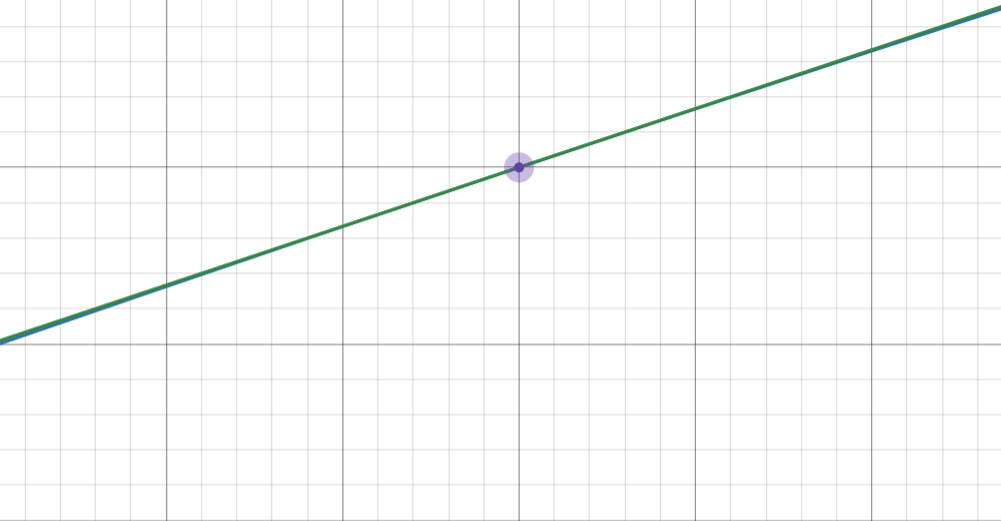
\includegraphics[width=0.5\linewidth]{2.png}
\end{figure}
\subsection{}
The tangent line's slope at \(t = 4\) represents the object's instantaneous velocity at that moment. We want to take the limit for a general \(t\) to find the equation of the rate of change of position. 

\[v(t) = \lim_{h \to0} \frac{s(t+h) - s(t)}{h} = \lim_{h\to0} \frac{\sqrt{2(t+h)+1} - \sqrt{2t+1}}{h}\]
\[= \lim_{h\to0} \frac{2}{\sqrt{2(t+h)+1} +\sqrt{2t+1} } = \frac{2}{2\sqrt{2t+1}} = \frac{1}{\sqrt{2t+1}}\]
We can see that as \(t\) increases, the velocity decreases as \(\frac{1}{\sqrt{2t+1}}\) decreases. Hence it slows down over time. 




\end{document}